\documentclass[mat1, tisk]{fmfdelo}
% \documentclass[fin1, tisk]{fmfdelo}
% Če pobrišete možnost tisk, bodo povezave obarvane,
% na začetku pa ne bo praznih strani po naslovu, …

%%%%%%%%%%%%%%%%%%%%%%%%%%%%%%%%%%%%%%%%%%%%%%%%%%%%%%%%%%%%%%%%%%%%%%%%%%%%%%%
% METAPODATKI
%%%%%%%%%%%%%%%%%%%%%%%%%%%%%%%%%%%%%%%%%%%%%%%%%%%%%%%%%%%%%%%%%%%%%%%%%%%%%%%

% - vaše ime
\avtor{Simon Grad}

% - naslov dela v slovenščini
\naslov{Izračun števila prirejanj v katakondenziranih benzenoidnih sistemih}

% - naslov dela v angleščini
\title{Computing the Number of Matchings in
Catacondensed Benzenoid Systems}

% - ime mentorja/mentorice s polnim nazivom:
%   - doc.~dr.~Ime Priimek
%   - izr.~prof.~dr.~Ime Priimek
%   - prof.~dr.~Ime Priimek
%   za druge variante uporabite ustrezne ukaze
\mentor{prof.~dr.~Sandi Klavžar}
% \somentor{...}
% \mentorica{...}
% \somentorica{...}
% \mentorja{...}{...}
% \somentorja{...}{...}
% \mentorici{...}{...}
% \somentorici{...}{...}

% - leto diplome
\letnica{2023} 

% - povzetek v slovenščini
%   V povzetku na kratko opišite vsebinske rezultate dela. Sem ne sodi razlaga
%   organizacije dela, torej v katerem razdelku je kaj, pač pa le opis vsebine.
\povzetek{V diplomskem delu
je obravnavana tematika iz področja kemijske teorije grafov.
Hosoyev indeks (Z indeks) grafa $G$ je definiran kot 
$Z(G) = \sum_{k \geq 0} p(G,k)$, 
kjer $p(G,k)$ označuje število $k$-prirejanj v grafu $G$, 
in je povezan z mnogimi termodinamičnimi lastnostmi
kot so vrelišče, entropija in skupna $\pi$-elektronska energija.
Cilj diplomskega dela je s pomočjo matrik predstaviti način,
kako lahko izračunamo 
Hosoyev indeks v poljubnem katakondenziranem benzenoidnem sistemu.}

% - povzetek v angleščini
\abstract{The thesis 
deals with topics from the field of chemical graph theory. 
The Hosoya index of a graph $G$ is defined as
${Z(G) = \sum_{k \geq 0} p(G,k)}$,
where $p(G,k)$ is the number of $k$-matchings in the graph $G$,
and is associated with many thermodynamic properties
such as boiling point, entropy and total $\pi$-electron energy.
The aim of this thesis is to present a way
to compute the Hosoya index of catacondensed benzenoid systems
with transfer matrix technique.}

% - klasifikacijske oznake, ločene z vejicami
%   Oznake, ki opisujejo področje dela, so dostopne na strani https://www.ams.org/msc/
\klasifikacija{..., ...}

% - ključne besede, ki nastopajo v delu, ločene s \sep
\kljucnebesede{...\sep ...}

% - angleški prevod ključnih besed
\keywords{...\sep ...} % angleški prevod ključnih besed

% - angleško-slovenski slovar strokovnih izrazov
\slovar{
% \geslo{angleški izraz}{slovenski izraz}
% ...
}

% - ime datoteke z viri (vključno s končnico .bib), če uporabljate BibTeX
% \literatura{....bib}

%%%%%%%%%%%%%%%%%%%%%%%%%%%%%%%%%%%%%%%%%%%%%%%%%%%%%%%%%%%%%%%%%%%%%%%%%%%%%%%
% DODATNE DEFINICIJE
%%%%%%%%%%%%%%%%%%%%%%%%%%%%%%%%%%%%%%%%%%%%%%%%%%%%%%%%%%%%%%%%%%%%%%%%%%%%%%%

% naložite dodatne pakete, ki jih potrebujete
% \usepackage{...}
\usepackage{graphicx}
\usepackage{subcaption}
\usepackage{float}
\usepackage{tikz}
\usepackage{arydshln}
\usetikzlibrary{positioning}

% deklarirajte vse matematične operatorje, da jih bo LaTeX pravilno stavil
% \DeclareMathOperator{\...}{...}
\def\N{\mathbb{N}} % mnozica naravnih stevil
\def\Z{\mathbb{Z}} % mnozica celih stevil
\def\Q{\mathbb{Q}} % mnozica racionalnih stevil
\def\R{\mathbb{R}} % mnozica realnih stevil
\def\C{\mathbb{C}} % mnozica kompleksnih stevil

% vstavite svoje definicije ...
% \newcommand{\...}{...}

%%%%%%%%%%%%%%%%%%%%%%%%%%%%%%%%%%%%%%%%%%%%%%%%%%%%%%%%%%%%%%%%%%%%%%%%%%%%%%%
% ZAČETEK VSEBINE
%%%%%%%%%%%%%%%%%%%%%%%%%%%%%%%%%%%%%%%%%%%%%%%%%%%%%%%%%%%%%%%%%%%%%%%%%%%%%%%

\begin{document}

\section{Uvod}
Teorija grafov preučuje objekte, ki se imenujejo grafi.
V matematiki je graf $G$ urejeni par množice vozlišč in povezav med njimi. 
Označimo ga $G = (V,E)$, kjer je $V$ neprazna množica vozlišč in $E$ množica povezav.
Vozlišča in povezave lahko 
predstavljajo veliko različnih objektov in relacij med njimi.
Vozlišča so lahko vse od ljudi, podjetij, avtobusnih postaj 
do oglikovih atomov. V delu bomo enačili:

\begin{itemize}
  \item graf = skeletna formula molekule,
  \item vozlišče = ogljikov(C) atom,
  \item  poveza = kemijska (C-C) vez.
\end{itemize}













\section{Orodja teorije grafov}
V poglavju pred nami je podanih nekaj osnovnih definicij in izrekov iz teorije grafov,
kateri nas bodo spremljali skozi delo.


Za motivacijo prirejanj si poglejmo naslednji problem.
V množici ljudi na plesišču 
so nekateri plesalci kompatibilni med sabo. 
Pod kakšnimi pogoji si lahko vsak najde soplesalca, s katerim je kompatibilen? 

\begin{definicija}
  \emph{Prirejanje} v grafu $G$ je množica povezav $G$, v kateri noben par povezav nima skupnega krajišča.
\end{definicija}

\begin{zgled}

    Na sliki \ref{fig:plesisce} so štirje pleaslci in štiri pleaslke.
    Povezava med plesalcem in plesalko predstavlja njuno kompatibilnost.
    


\begin{figure} [H]
  \begin{center}

    \input{slike/plesisce.sty}
    \label{fig:plesisce}
    \caption{Graf plesalcev z enim od prirejanj.}
  \end{center}
\end{figure}

Prirenjanje na sliki označujejo odebeljene povezave, ki 
    vsakemu plesalcu priredijo soplesalko in obratno.
    Takemu prirejanju bomo rekli $4$-prirejanje, ker 
    vsebuje štiri povezave.
    Poleg tega pa ima vsak svojega soplesalca (nihče ni ostal brez soplesalca),
    kar pomeni, da je prirejanje na sliki popolno.
\end{zgled}

\begin{definicija}
  Prirejanju z močjo k bomo rekli \emph{$k$-prirejanje}.
\end{definicija}

%/V primeru zgoraj imamo 5-prirejanje. Saj smo določili 5 parov.

\begin{definicija}
  Če je $k$ tak, 
  da $k$-prirejanje grafa $G$ obstaja, 
  $k+1$-prirejanje pa ne, 
  potem rečemo $k$-prirejanju 
  tudi \emph{največje prirejanje} grafa $G$.
\end{definicija}
\begin{definicija}
  \emph{Popolno prirejaje} grafa je prirejanje, v katerem je vključeno vsako vozlišče.
\end{definicija}

\begin{definicija}
    \emph{$p(G,k)$} označuje število $k$-prirejanj v grafu $G$.
\end{definicija}


\begin{zgled}
    Recimo da imamo štiri pleaslce in štiri plesalke, 
    ki so vsi med sabo kompatibilni (glej sliko \ref{fig:plesisce2}).
    Grafu na sliki rečemo polni dvodelni graf in ga označimo s $K_{4,4}$.
    Očitno je, 
    da lahko vsakemu plesalcu priredimo soplesalko in obratno,
    oziroma v jeziku prirejanj, da lahko najdemo $4$-prirejanje.
    Postavimo si vprašanje, koliko je različnih $4$-prirejanj
    v našem grafu oziroma na koliko različnih načinov lahko 
    poparčkamo plesalce.
    
    Ker lahko vsak pleše z vsakim pomeni, da ima prvi plesalec 
    možnost izbirati med vsemi štirimi dekleti, drugi med tremi, tretji med dvema
    in zadnji nima izbire.
    To pomeni, da je število različnih $4$-prirejanj v grafu $K_{4,4}$
    enako $4!$, kar je $24$ različnih načinov na katere lahko poparčkamo
    plesalce med sabo.

    $$p(K_{4,4},4) = 4! = 24$$

\begin{figure} [H]
    \begin{center}
  
      \input{slike/plesisce2.sty}
      \label{fig:plesisce2}
      \caption{Graf plesalcev.}
    \end{center}
  \end{figure}

  Podobno bi veljalo tudi, če bi imeli $n$ plesalcev
  in $n$ plesalk. 
  $$p(K_{n,n},n) = n! $$
\end{zgled}


Očitno je, da je vsako popolno prirejanje tudi največje.

Popolni prirejanji v šestkotniku sta dve (glej sliko \ref{fig:benzen})
in ponazarjata dve enakovredni formuli benzena, 
ki dopuščata spreminjanje položaja dvojnih vezi.
Molekula benzena ves čas prehaja iz ene 
 v drugo obliko.

Danes se najpogosteje za prikazovanje prostih $\pi$-elektronov
uporablja model Kekuléjevih struktur. 
Te prikazujejo dvojne vezi v strukturni formuli, ki
pa morajo biti postavljene tako, da ima
vsak ogljikov atom natanko eno dvojno vez.
V jeziku prirejanj, to pomeni, da bo število
vseh Kekuléjevih struktur za neko benzenoidno molekulo,
kar enako številu različnih popolnih prirejanj te molekule.


\begin{figure}[H]
  \centering
  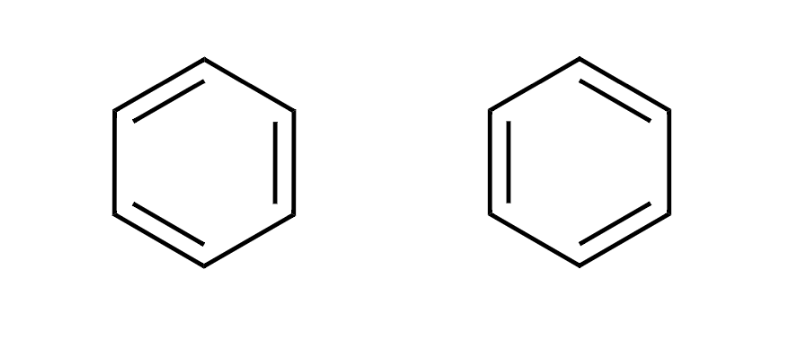
\includegraphics[width = 0.5 \textwidth]{slike/benzena.png}
  \caption{Kekuléjevi strukturi benzena}
  \label{fig:benzen}
\end{figure}


Iz slike \ref{fig:benzen} vidimo, da je
$p(C_6,3) = 2$, saj obstajata v grafu $G$ natanko
dva $3$-prirejanja.
Za rezultate o računanju števila prirejanj nekaterih grafov glej \cite{4-pri}. 














\section{Benzenoidni sistemi}

Obravnavana tematika v tem razdelku sega na področje organske kemije, 
zato si najprej oglejmo nekaj osnov policikličnih aromatskih oglikovodikov, 
saj so ti motivacija za vpeljavo benzenoidnih (heksagonalnih) sistemov.

Benzen $C_6 H_6$ je prototip aromatskih spojin, ki so nenasičene spojine
z nizko stopnjo reaktivnosti. Gre za ravninsko molekulo, 
ki se pojavi v obliki popolnega šestkotnika s stranico oziroma
C-C vezjo dolgo $0.139$ nm. Kot že omenjeno v prvem razdelku  
je benzen hibrid dveh ekvivalentnih
(Kekuléjevih) struktur, ki se razlikujeta zgolj v lokaciji dvojnih vezi (glej sliko \ref{fig:benzen}).
To je zgolj ena od ponazoritev 
delokaliziranih $\pi$-elektronov, 
kateri zaradi prekrivanja $2p$ orbital dajejo molekuli večjo stabilnost. 
Če je več obročev benzena povezanih med seboj, govorimo o policikličnih
aromatskih oglikovodikih.
Znan primer je naftalen (glej sliko \ref{fig:naftalen-kot-benzenoidni}). 


\begin{figure}[ht!]
    \centering
    \includegraphics[width = 0.9 \textwidth]{slike/kemija-benzenoidni.png}
    \caption{(a)Naftalen (b)Predstavitev naftalena kot benzenoidni sistem}
    \label{fig:naftalen-kot-benzenoidni}
\end{figure}



% del kemijski teoriji grafov? kako se navezuje kemija na tg

Benzenoidni sistemi so matematični model za preučevanje policikličnih aromatskih ogljikovodikov.
Kot je benzen osnovni gradnik policikličnih aromatskih ogljikovodikov, 
je osnovni gradnik benzenoidnih sistemov pravilni šestkotnik,
katerega koti bodo veljali za vozlišča grafa in stranice za povezave grafa.
Benzenoidni sistem je definiran na neskončni mreži v ravnini 
sestavljeni iz samih pravilnih šestkotnikov, kot kaže slika \ref{fig:benzenoidni-sistem}.
Sklenjeni krivulji, ki poteka po stranicah šestkotnikov, bomo rekli cikel.

\begin{figure}[ht!]
    \centering
    \begin{subfigure}{.5\textwidth}
      \centering
      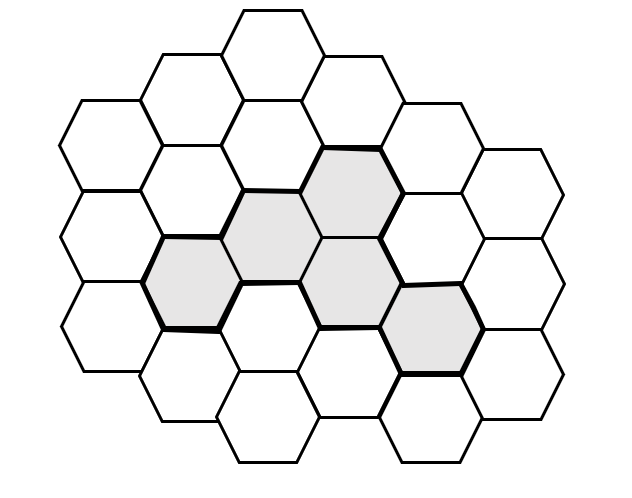
\includegraphics[width=.9\linewidth]{slike/benzenoidni-sistem-cb.png}
      \caption{Cikel na mreži šestkotnikov}
    \end{subfigure}%
    \begin{subfigure}{.5\textwidth}
      \centering
      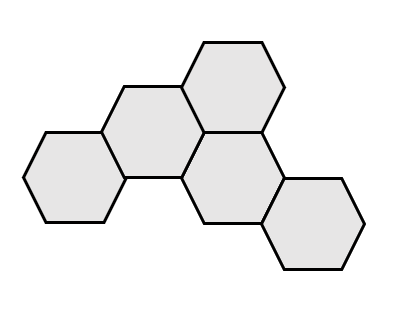
\includegraphics[width=.9\linewidth]{slike/benzenoidni.png}
      \caption{Pripadajoči benzenoidni sistem}
    \end{subfigure}
    \caption{Benzenoidni sistem}
    \label{fig:benzenoidni-sistem}
\end{figure}  


\begin{definicija}
  Naj bo C cikel na šestkotni mreži. \emph{Benzenoidni sistem} je sestavljen 
  iz vseh vozlišč in povezav, ki ležijo v njegovi notranjosti ali na ciklu C.
   (Glej sliko \ref{fig:benzenoidni-sistem})
\end{definicija}

Vozlišča benzenoidnega sistema, ki niso del cikla, imenujemo \emph{notranja vozlišča}.

\begin{definicija}
  Benzenoidni sistem je \emph{katakondenziran benzenoidni sistem}, če ne vsebuje notranjih vozlišč,
  sicer je \emph{perikondenziran benzenoidni sistem}.
   (Glej sliko \ref{fig:peri-kata})
\end{definicija}

\begin{figure}[ht!]
  \centering
  \begin{subfigure}{.5\textwidth}
    \centering
    \includegraphics[width=.9\linewidth]{slike/perikondenziran_z_notranjim_voziscem.png}
    \caption{Perikondenziran}
    \label{fig:sub1}
  \end{subfigure}%
  \begin{subfigure}{.5\textwidth}
    \centering
    \includegraphics[width=.9\linewidth]{slike/katakondenziran-sistem.png}
    \caption{Katakondenziran}
    \label{fig:sub2}
  \end{subfigure}
  \caption{Tipa benzenoidnih sistemov}
  \label{fig:peri-kata}
\end{figure}


% Še druga definicija za peri in kata kndenzirane z duali??







\section{Hosoyev indeks}

To poglavje namenimo povezavi med kemijo in teorijo grafov. 
Seznanimo se z topološkimi indeksi in bolj podrobno ogledamo 
Hosoyev indeks.

\begin{definicija}
    \emph{Topološki indeks} je funkcija, ki grafu priredi število in
    predstavlja grafovsko invarianto.
\end{definicija}

V kemiji je znanih že mnogo topoloških indeksov.
Klasificiramo jih lahko po strukturnih lastnostih grafov, 
ki se uporabljajo za njihov izračun.
Na primer, Wienerjev indeks temelji na razdalji vozlišč v grafu, 
Randičev indeks na stopnji vozlišč,
Hosoyev indeks pa na številu prirejanj v grafu.

Topološki indeksi se pogosto uporabljajo v kemiji
za preučevanje lastnosti molekule. 
V primeru Hosoyevega indeksa ima ta določeno
korelacijo med strukturo spojine in njenimi 
termodinamičnimi lastnostmi.

Uporaba topoloških indeksov v biologiji in kemiji 
se je začela leta 1947, ko je kemik Harold Wiener
uvedel tako imenovani Wienerjev indeks. 
Haruo Hosoya je leta 1971 v članku \cite{HOSOYA}
predstavil nov indeks imenovan Z indeks.
Ta povezuje mnoge termodinamične lastnosti molekule
s številom prirejanj.
S časom se je 
Z indeks preimenoval
kar v  Hosoyev indeks po avtorju indeksa.
   
\begin{definicija}
    \emph{Hosoyev indeks} grafa G je definiran kot
    $$
    Z(G) = \sum_{ k > 0} p(G,k),
    $$
    kjer je $k \in \N$.
\end{definicija}

Za motivacijo si oglejmo tri primere enostavnih
molekul in izračunajmo njihov Hosoyev indeks.

\begin{zgled}

  Izračunajmo Hosoyev indeks za propan, 2,2-dimetilpropan in pentan.

  Propan lahko enačimo z grafom $P_3$ to je pot dolžine 3 (glej sliko \ref{fig:propan}). 
  Zanima nas torej Hosoyev indeks grafa $P_3$.  
  Izračunati moramo torej 
  $$Z(P_3) = p(P_3,1) + p(P_3,2) + p(P_3,3) + \dots$$

  $p(P_3,1)$ označuje koliko je različnih $1$-prirejanj v grafu $P_3$.
  To bo kar enako številu vseh povezav grafa, kar pomeni da je
  $p(P_3,1) = 2$.

  Hitro ugotovimo, da je za vsak $k \geq 2$ 
  $p(P_3,k) = 0$, saj na grafu $P_3$ $2$-prirejanje ne obstaja.
  
  
  \begin{figure} [H]
    \begin{center}
  
      \input{slike/propan.sty}
      \label{fig:propan}
      \caption{Propan.}
    \end{center}
  \end{figure}


  Podoben postopek naredimo za 2,2-dimetilpropan (glej sliko \cite{fig:dimetilpropan}).
  
  $p(2,2-dimetilpropan, 1) = 4$, 
  za $k \geq 2$ pa velja
  $p(2,2-dimetilpropan, k) = 0$.
  \begin{figure} [H]
    \begin{center}
  
      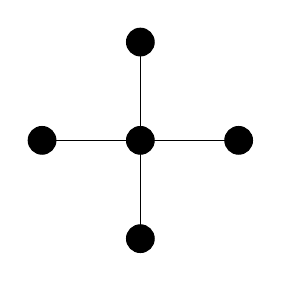
\begin{tikzpicture}[
    youngnode/.style={rectangle, draw=red!60, fill=red!5, very thick, minimum size=40},
    oldnode/.style={rectangle, draw=blue!60, fill=blue!5, very thick, minimum size=40},
    ]
      %Nodes
      \node      (A)                         {};
      \node      (B)       [right=of A]      {};
      \node      (C)       [right=of B]      {};
      % \node      (D)       [right=of C]      {};
      % \node      (E)       [right=of D]      {};
    
      % \node      (M)        [below=of A]      {};
      \node      (N)        [below=of B]      {};
      % \node      (O)        [below=of C]      {};
      % \node      (P)        [below=of D]      {};
      \node      (R)        [above=of B]      {};
    
      \filldraw [black] (A) circle (5pt); 
      \filldraw [black] (B) circle (5pt); 
      \filldraw [black] (C) circle (5pt); 
      % \filldraw [black] (D.south) circle (5pt); 
    
      % \filldraw [black] (M.north) circle (5pt); 
      \filldraw [black] (N) circle (5pt); 
      % \filldraw [black] (O.north) circle (5pt); 
      % \filldraw [black] (P.north) circle (3pt); 
      \filldraw [black] (R) circle (5pt);
  
      %Lines
      % \draw[-, ultra thin] (A.south)  to node[right] {} (M.north);
      % \draw[-, ultra thin] (A.south)  to node[right] {} (N.north);
      % \draw[-, ultra thin] (A.south)  to node[right] {} (O.north);
      % \draw[-, ultra thin] (A.south)  to node[right] {} (P.north);
    
      % \draw[-, ultra thin] (B.south)  to node[right] {} (M.north);
      \draw[-, ultra thin] (B.south)  to node[right] {} (N.north);
      \draw[-, ultra thin] (B.west)  to node[right] {} (A.east);
      \draw[-, ultra thin] (B.east)  to node[right] {} (C.west);

      \draw[-, ultra thin] (R.south)  to node[right] {} (B.north);
      % \draw[-, ultra thin] (B.south)  to node[right] {} (O.north);
      % \draw[-, ultra thin] (B.south)  to node[right] {} (P.north);

      % \draw[-, ultra thin] (C.south)  to node[right] {} (M.north);
      % \draw[-, ultra thin] (C.south)  to node[right] {} (N.north);
      % \draw[-, ultra thin] (C.south)  to node[right] {} (O.north);
      % \draw[-, ultra thin] (C.south)  to node[right] {} (P.north);

      % \draw[-, ultra thin] (D.south)  to node[right] {} (M.north);
      % \draw[-, ultra thin] (D.south)  to node[right] {} (N.north);
      % \draw[-, ultra thin] (D.south)  to node[right] {} (O.north);
      % \draw[-, ultra thin] (D.south)  to node[right] {} (P.north);
      % \draw[-, ultra thin] (D.south)  to node[right] {} (R.north);
    \end{tikzpicture}
      \label{fig:dimetilpropan}
      \caption{2,2-dimetilpropan.}
    \end{center}
  \end{figure}


  In še za pentan (glej sliko \cite{fig:pentan}), ki ga lahko
  enačimo z grafom $P_5$. 
  Velja $p(P_5, 1) = 4$ in $p(P_5, 2) = 3$ torej je $Z(P_5) = 4 + 3 = 7$.
  Na sliki \cite{fig:pentan} so z odebeljenimi
  povezavami ponazorjena vsa različna $2$-prirejanja grafa $P_5$.


  \begin{figure} [H]
    \begin{center}
      \begin{tabular}{@{}cccc@{}}
        {\input{slike/pentan1.sty}} \\ 
        {\input{slike/pentan2.sty}} \\ 
        \input{slike/pentan3.sty}
      \end{tabular}

      \label{fig:pentan}
      \caption{$2$-prirejanja pentana}
    \end{center}
  \end{figure}


  Kot smo izračunali ima od naštetih primerov najmanjši Hosoyev indeks
  propan, največjega pa ima pentan. Ta podatek lahko hitro povežemo tudi z
  mnogimi termodinamičnimi lastnostmi, kot je na primer vrelišče spojine.
  Saj ima od naštetih propan najnižje vrelišče in pentan najvišje.
  V kemiji je splošno znano dejstvo, da se z dodajanjem oglikovih atomov 
  (v teoriji grafov so to vozlišča) vrelišče spojine povečuje in da imajo 
  razvejane molekule (2,2-dimetilpentan) nižje vrelišče 
  od nerazvejanih (pentan), čeprav imajo isto število ogljikovih atomov.
\end{zgled}









\section{Izračun števila prirejanj v katakondenziranih benzenoidnih sistemih}

% V tem poglavju bomo izpolnili še najpomembnejši cil dimplomskega dela:
% izračunali bomo število prirejanj v katakondenziranih benzenoidnih sistemih.
% Najprej bomo navedli dve pomembni lemi (rekurzivni formuli), 
% ki nam bosta pomagali priti do števila prirejanj.
% Kasneje bomo z uvedbo vektorja 
% $p_{ab}(G,k)$ in množenjem z ustreznimi matrikami izračunali 
% Hosoyev indeks.
% Oznake in leme tega poglavja so povzete 
% po \cite{GLAVNA DIPLOMSKA} in \cite{GLAVNA DIPLOMSKA}.

V tem poglavju se lotimo naslovnega problema:
"Kako izračunati število $k$-prirejanj v poljubnem katakondenziranem benzenoidnem sistemu."
Najprej bomo zaradi zanimivosti in motivacije 
navedli nekaj enostavnejših primerov, 
katakondenziranih sistemov, kjer
znamo število prirejanj hitro izračunati.
Nato pa se bomo osredotočili na povsem splošen primer.
Za katerega bomo navedli dve pomembni lemi (rekurzivni formuli), 
ki nam bosta pomagali priti do števila prirejanj.
Kasneje bomo z uvedbo vektorja 
$p_{ab}(G,k)$ in množenjem z ustreznimi matrikami izračunali 
Hosoyev indeks.
Oznake in leme tega poglavja so povzete 
po \cite{GLAVNA DIPLOMSKA} in \cite{GLAVNA DIPLOMSKA}.


Par konkretnik primerov, če nas zanima število $k$-prirejanj 
v poljubnih grafih za specifičen $k$.
Če $k = 0$, za poljuben graf $G$ velja, da je $p(G,0) = 1$.
Če $k = 1$, za poljuben graf $G$ z velja, da je $p(G,1) = |E|$.

Obstajajo tudi posebni primeri benzenoidnih sistemov, 
v katerih lahko hitro izračunamo število popolnih prirejanj $p(G, 2n+1)$.
Moč množice prirejanj je v benzenoidnem sistemu z $n$ šestkotniki $2n+1$.

\begin{zgled}
  Tak primer so linearne benzenoidne verige, 
  za katere velja 
  $$p(G, 2n + 1) = n + 1$$.
  \begin{figure}[H]
    \centering
    \includegraphics[width = 0.5 \textwidth]{slike/linearna_veriga.png}
    \caption{ Linearna benzenoidna veriga}
    \label{fig:linearna_veriga}
  \end{figure}
  Za molekulo na sliki \ref{fig:linearna_veriga}
  velja $
  p(G, 11) = 6
  $.
\end{zgled}




\begin{zgled}
  Še bolj zanimiv primer so \emph{fibonačeni}.
  To so benzenoidne verige z zig-zag strukturo 
  (to pomeni, da trije zaporedni šestkotniki ne smejo ležati na isti premici).
  Ponujajo matematično zanimivo strukturo za več %[referenca na članek]
  Kot že njihovo ime namiguje v njih najdemo Fibonačijevo zaporedje
  ($F_0 = 1$, $F_1 = 1$, $F_2 = 2$, $F_3 = 3$, $F_4 = 5$ ...). 
  
  Za fibonačene velja 
  \begin{equation}
    p(G ,2n+1) = F_{n+1}.
    \label{eq:fibonaceni}
  \end{equation}
  
  \begin{figure}[H]
    \centering
    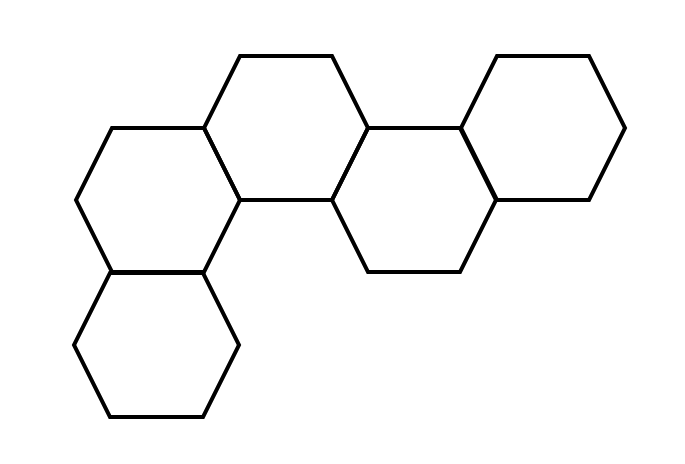
\includegraphics[width = 0.5 \textwidth]{slike/fibonacin.png}
    \caption{Fibonačen}
    \label{fig:fibonaceni}
  \end{figure}
  Za molekulo na sliki \ref{fig:fibonaceni}
  ima $5$ šestkotnikov in ustreza obliki fibonačenov, saj je benzenoidna veriga
  z zig-zag strukturo. Po formuli ima molekula $F_{5+1} = 13$ popolnih prirejanj.
  Sepravi lahko zapišemo
  $
  p(G, 11) = 13
  $.
\end{zgled}

V zgledu smo formulo \ref{eq:fibonaceni} zgolj privzeli za znano.
Spodobi se, da jo tudi dokažemo.

\noindent
{\em Dokaz:\/}[Fibonačeni]
Dokaz bomo bomo naredili s pomočjo matematične indukcije po številu šestkotnikov v danem
fibonačenu. Naj $n$ označuje število šestkotnikov.

\emph{ $n = 1$ :} Izračunati moramo število popolnih prirejanj v šestkotniku. 
To smo že naredili na sliki \ref{fig:benzen}. Torej velja 
$p(G,2n+1) = p(G,3) = 2 = F_{2} = F_{n+1}$.

\emph{ $n = 2$ :} 
Iz slike \ref{fig:naftalen} vidimo, da formula velja tudi 
za $n = 2$. 
Torej $p(G,2n+1) = p(G,5) = 3 = F_{3} = F_{n+1}$.
\begin{figure}
  \centering
  \includegraphics[width = 0.5 \textwidth]{slike/naftalen.png}
  \caption{Vsa možna popolna prirejanja naftalena.}
  \label{fig:naftalen}
\end{figure}


\emph{$(n)$ in $(n-1) \Rightarrow (n+1)$ :}
Naj bo $G$ graf z $n+1$ šestkotniki. Uporabimo izrek %referenca
, da velja $p(G,k) = p(G-ab,k) + p(G-a-b, k-1)$. Kjer sta $a$ in $b$
poljubni vozlišči v $G$.

Za $a$ in $b$ si izberimorobni vozlišči

\qed


Sedaj se osredotočimo na splošen primer,
ki ga bomo rešili s pomočjo rekurzije.
Najprej navedemo dve pomembni lemi (rekurzivni formuli)
s katerima bomo dokazali kasnejše izreke. 

\begin{lema}
  Naj bosta $a$ in $b$ vozlišči v grafu $G$, povezava med njima pa $ab$.
  Velja
    $$p(G,k) = p(G-ab,k) + p(G-a-b, k-1) $$
    \label{lema1}
\end{lema}
\begin{proof}
  Lemo dokažemo s kratkim razmislekom.
  $p(G,k)$ označuje število vseh različnih
  $k$-prirejanj v grafu $G$. 
  Povezava $ab$ je lahko v prirejanju ali pa je ni v prirejanju.
  Število različnih $k$-prirejanj b $G$, ki ne vsebujejo povezave $ab$,
  je $p(G-ab,k)$,število tistih, ki vsebujejo povezavo $ab$ pa $p(G-a-b, k-1)$.
  
  S tem je lema dokazana.
\end{proof}

\begin{lema}
  Naj bo $G$ graf za katerega velja $G = H \cup S$, 
  kjer sta $H$ in $S$ komponenti grafa $G$. Velja
  $$
  p(H \cup S, k) = p(H,k)p(S,0) + p(H,k-1)p(S,1) + \dots + p(H,0)p(S,k). 
  $$
  \label{lema2}
\end{lema}
\begin{proof}
  Ker imamo dve komponenti grafa $G$, ki med sabo nista povezani in
  iščemo število različnih $k$-prirejanj v grafu $H \cup S$,
  lahko $p(H \cup S, k)$ zapišemo kot vsoto različnih možnosti.
  Prva možnost bo, da najdemo kar $k$-prirejanje v grafu $H$ ($p(H,k)p(S,0)$),
  druga da najdemo v $H$ $k-1$-prirejanje in v $S$ $1$-prirejanje ($p(H,k-1)p(S,1)$)\dots
\end{proof}


Definiramo vektor $k$-prirejanja na $G$ definiran na povezavi $ab$. 

\begin{definicija}
  Naj bo $G$ graf in ab povezava grafa $G$.
  \emph{Vektor $k$-prirejanja} grafa $G$ v povezavi $ab$ je definiran kot 
  $$p_{ab}(G,k) =
  \tiny
  \begin{pmatrix}
     p(G,k) \\
     p(G,k-1) \\
     \vdots \\
     p(G, 1) \\
     p(G, 0) \\
     p(G - a, k) \\
     p(G - a, k-1) \\
     \vdots \\
     p(G - a, 1) \\
     p(G - a, 0) \\
     p(G - b, k) \\
     p(G - b, k-1) \\
     \vdots \\
     p(G - b, 1) \\
     p(G - b, 0) \\
     p(G - a - b, k) \\
     p(G - a - b, k-1) \\
     \vdots \\
     p(G - a - b, 1) \\
     p(G - a - b, 0) \\
  \end{pmatrix} $$
\end{definicija}

Hitro ugotovimo, da če poznamo ta vektor za povezavo $ab$, 
poznamo tudi število $k$-prirejanj v grafu $G$ za poljuben $k$ 
(in vsa $l$-prirejanja, kjer je $l$ manjši od $k$).

%POZOR: DELITEV NA GOR DOL NARAVNOST IN LOČENO

Z uporabo naslednjih izrekov uspemo z 
matričnim množenjem in redukcijo izračunati iskani vektor.
To naredimo na način, da vektor $p_{ab}(G,k)$ rekurzivno premaknemo 
na $p_{ij}(S,k)$, kjer je $S \subset G$. 
Premike lahko naredimo na štiri različne načine
odvisne od strukture benzenoidnega sistema.

\begin{figure}[h!]
  \centering
    \begin{subfigure}{.24\textwidth}
      \centering
      \includegraphics[width=.85\linewidth]{slike/linearno.png}
    \end{subfigure}%
    \begin{subfigure}{.24\textwidth}
      \centering
      \includegraphics[width=.83\linewidth]{slike/kot.png}
    \end{subfigure}
    \begin{subfigure}{.24\textwidth}
      \centering
      \includegraphics[width=.83\linewidth]{slike/kot2.png}
    \end{subfigure}
    \begin{subfigure}{.24\textwidth}
      \centering
      \includegraphics[width=.8\linewidth]{slike/krozisce.png}
    \end{subfigure}
  \caption{Tipi šestkotnikov v katakondenzitanih benzenoidnih sistemih}
  \label{fig:stiri_nacini}
\end{figure}
Sedaj bomo 
za vsakega od načinov na sliki \ref{stiri_nacini} 
zapisali izrek in ga dokazali.

\begin{figure}[h!]
  \centering
  \includegraphics[width = 0.4 \textwidth]{slike/rekurzivno_linearno.png}
  \caption{Graf v izreku \ref{izrek:1}}
  \label{fig:rekurzivno_linearno}
\end{figure}
\begin{izrek}
  Naj bo $G = (V, E)$ graf pridobljen s 
  spajanjem grafa $S$ in šestkotnika 
  v povezavi $de$ (glej sliko \ref{fig:rekurzivno_linearno}). Potem velja
  $$p_{ab}(G,k) = Q \cdot p_{cd}(S,k),$$
  kjer $Q$ predstavlja $4(k+1) \times 4(k+1)$ dimenzionalno matriko.  
  \begin{figure}[H]
    \centering
    \includegraphics[width = 0.8 \textwidth]{slike/matrika_Q.png}
    \label{fig:Q}
  \end{figure}
  \label{izrek:1}
\end{izrek}

\begin{dokaz}
  Za začetek si oglejmo prvo komponento $p_{ab}(G,k)$ to je  $p(G,k)$.
  Najprej dvakrat uporabimo lemo \ref{lema1} potem 
  preimenujemo graf, tako da namesto grafa $G$
  vsebuje graf $S$. Na primer namesto $G- cf - gd$ zapišemo
  $S \cup P_4$ (glej sliko \ref{graf_brez}). 
  Uporabimo lemo \ref{lema2} in opazimo, 
  da lahko vsoto zapišemo v obliki skalarnega produkta dveh vektorjev.
  \begin{align*} 
    p(G,k) &= p(G- cf - gd, k) + p(G- c-f - gd, k-1) 
      \\   &+ p(G- cf - g-d, k-1) +p(G- c-f - g-d, k-2)
      \\
      \\  &= p(S \cup P_4,k) + p((S-c) \cup P_3,k-1) 
      \\  &+ p((S-d) \cup P_3,k-1) + p((S-c-d) \cup P_2,k-2) 
      \\
      \\  &= p(S,k) \cdot p(P_4,0) + p(S,k-1) \cdot p(P_4,1) + p(S,k-2) \cdot p(P_4,2)
      \\  &+ p(S-c,k-1) \cdot p(P_3,0) + p(S-c,k-2) \cdot p(P_3,1)   
      \\  &+ p(S-d,k-1) \cdot p(P_3,0) + p(S-d,k-2) \cdot p(P_3,1)
      \\  &+ p(S-c-d,k-2) \cdot p(P_2,0) + p(S-c-d,k-3) \cdot p(P_2,1)
      \\
      \\  &= p(S,k) + 3p(S,k-1) + p(S,k-2)
      \\  &+ p(S-c,k-1)  + 2p(S-c,k-2)   
      \\  &+ p(S-d,k-1)  + 2p(S-d,k-2)
      \\  &+ p(S-c-d,k-2)  + p(S-c-d,k-3)
      \\
      \\ &= (1, 3, 1, 0, \dots ,0, \vdots 0, 0, 1, 2, 0, \dots, 0, \vdots 0, 1, 2, 0, \dots, 0, \vdots 0,0,1,1,0, \dots, 0) \cdot p_{cd}(S,k)
  \end{align*}
  \begin{figure}[h!]
    \centering
    \includegraphics[width = 0.4 \textwidth]{slike/linearni_brez.png}
    \caption{Graf $G- cf - gd$ oziroma $S \cup P_4$.}
    \label{fig:graf_brez}
  \end{figure}
  Številski vektor, ki smo ga dobili, ustreza prvi vrstici matrike $Q$.
  



\end{dokaz}









Z večkratno uporabo teh izrekov
prevedemo problem na izračun 
$p_{xy}(P_2,k)$, kjer je $P_2$ pot med preostalima vozliščema $x$ in $y$. 
Ta vektor pa znamo izračunati,
saj je vedno oblike
$$
p_{xy}(P_2,k) = [0 \dots 0 \quad 1 \quad 1 \quad 0 \dots 0 \quad 1 \quad 0 \dots 0 \quad 1 \quad 0 \dots 0 \quad 1].
$$
Na ta način lahko izračunamo število $k$-prirejanj v poljubnem katakondenziranem benzenoidnem sistemu.















\section{Zaključek}
...

\end{document}
